\section{Graph classes}

In our test protocols presented in the next section, we used various graph classes that we chose for their particular topology or for difficulties encountered in their coloration or to represent common cases used in research. All these types of graphs combined cover most of the existing types of graphs. Here are the types of graphs that we used:

\subsection{Chains}

\subsubsection{Odd number of vertices}

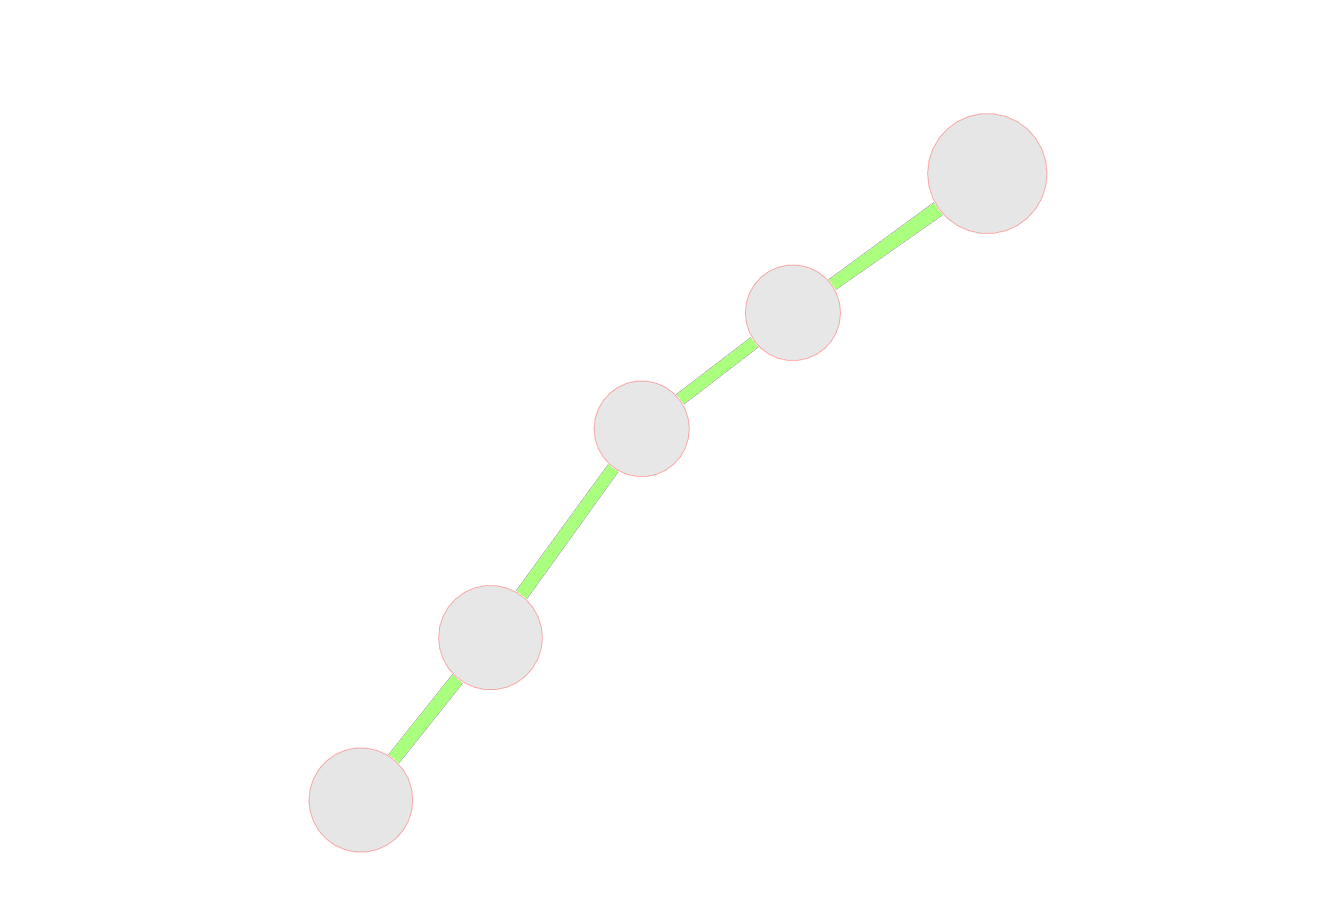
\includegraphics[width=11cm]{graphchaineimpaire.png}

\subsubsection{Even number of vertices}

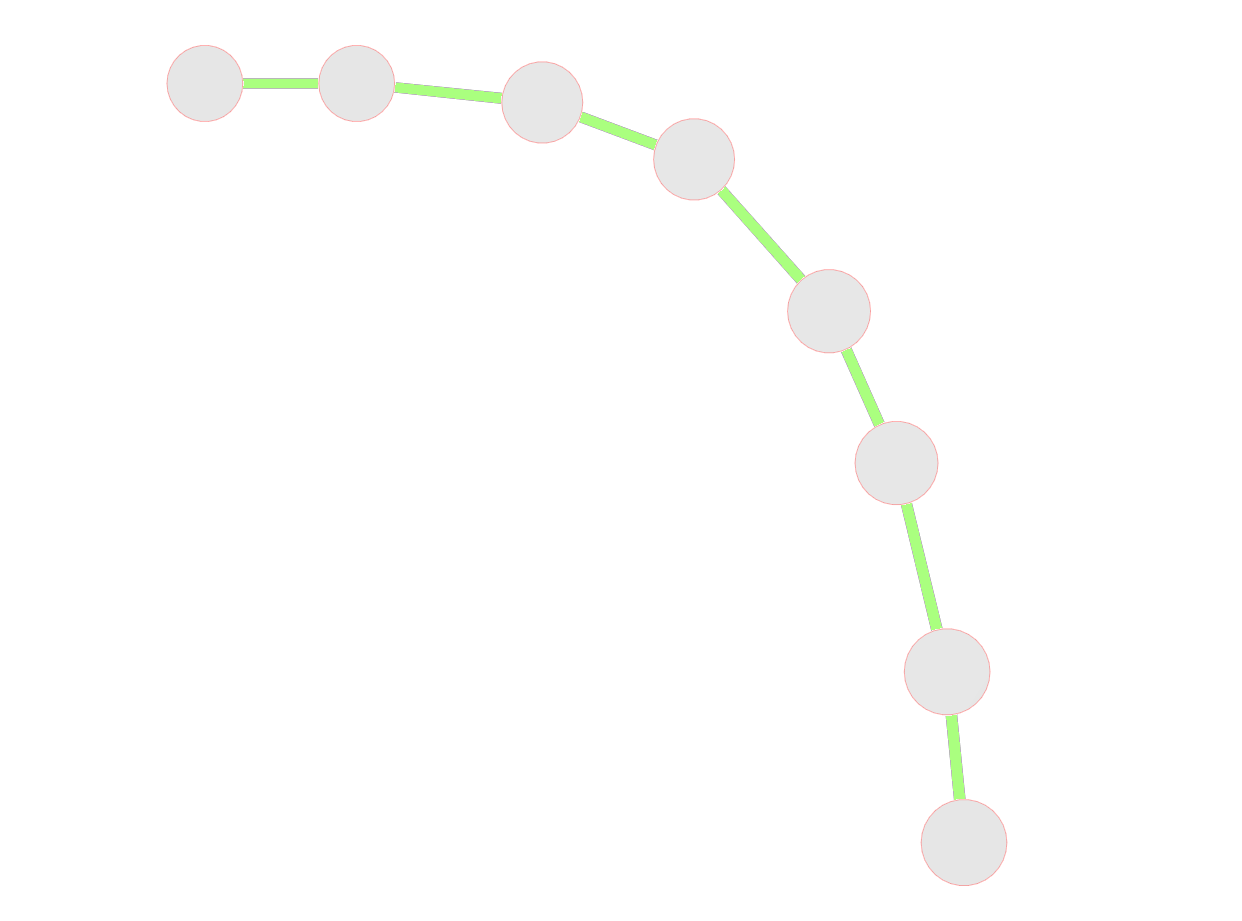
\includegraphics[width=11cm]{graphchainepaire.png}

The chains are 2-coloriable graphs. They regularly appear in problems that involve calculations of paths. In addition, they provide interesting examples both for their topology and their simplicity.

\subsection{Cycles}

\subsubsection{Odd number of vertices}

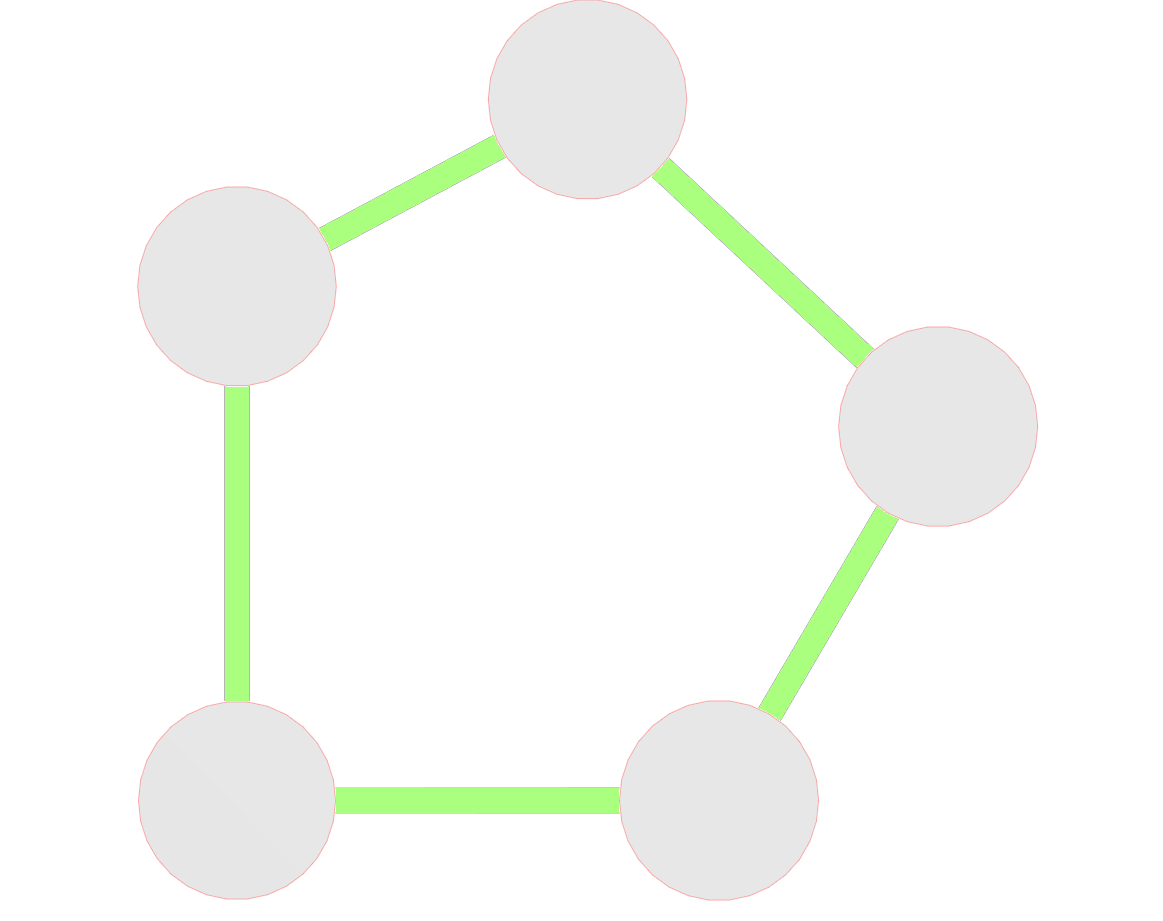
\includegraphics[width=11cm]{graphcycleimpair.png}

\subsubsection{Even number of vertices}

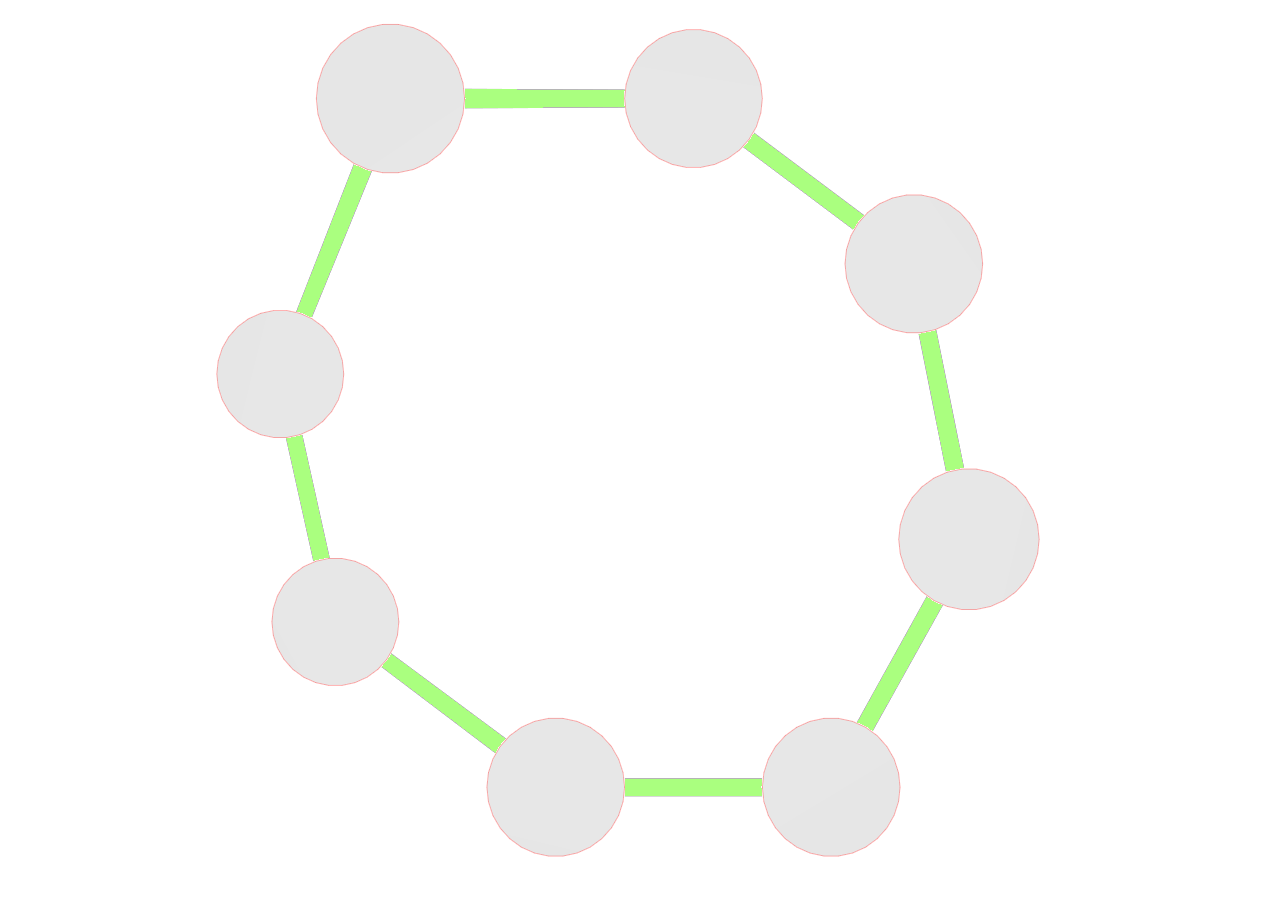
\includegraphics[width=11cm]{graphcyclepair.png}

Cycles are used in famous problems such as the traveling salesman problem. They particularly interest us since they form a direct link with the practical applications of graph coloring problems.

\subsection{Grids}

\subsubsection{2x5}

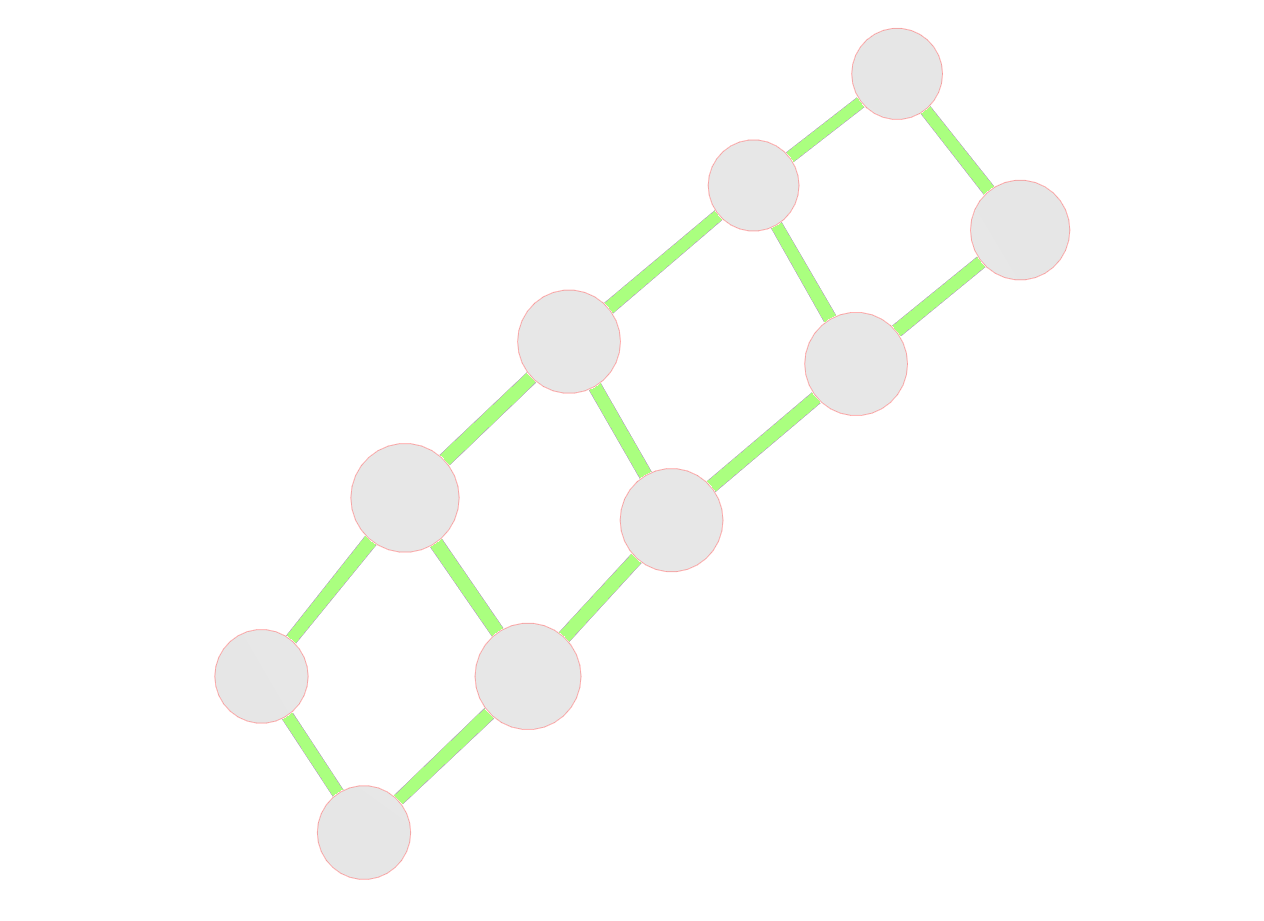
\includegraphics[width=11cm]{graphgrille25.png}

\subsubsection{5x5}

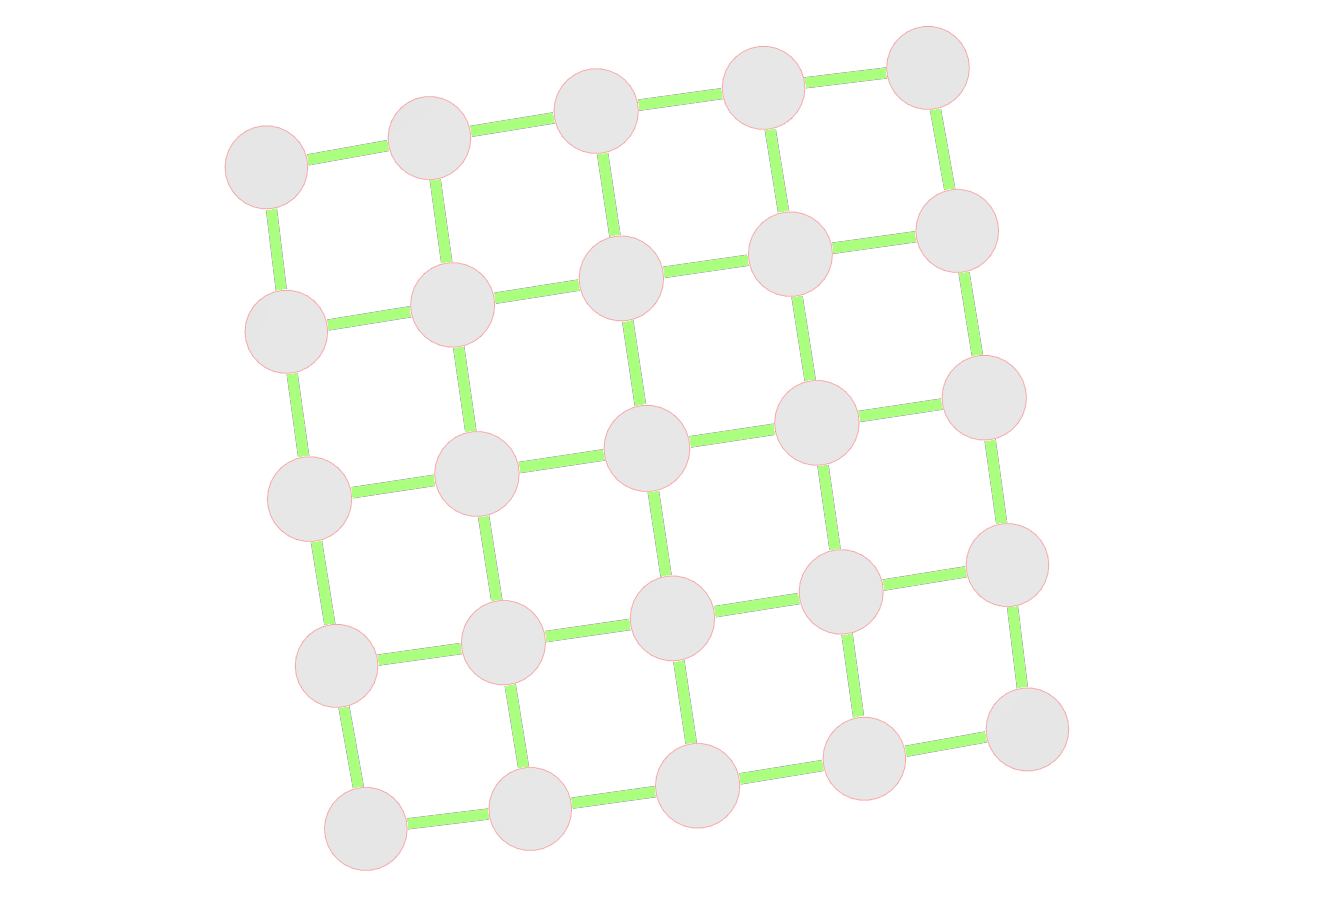
\includegraphics[width=11cm]{graphgrille55.png}

The grid is the type of graph which consumes the greatest amount of time in term of game simulation. This type of graph is mainly used in the fields of networking and communication.

\subsubsection{5x5 toroidal}

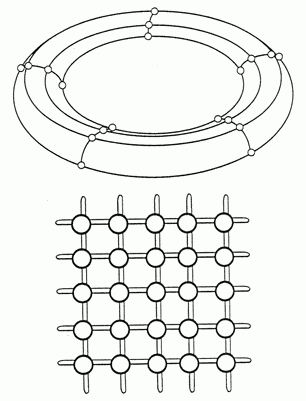
\includegraphics[width=11cm]{graphgrille55tor.png}

Toroidal grids are particularly relevant to the field of parallel computing. Similarly to conventional grids, they are difficult to exploit in our simulation algorithms.

\subsection{Binary Tree}

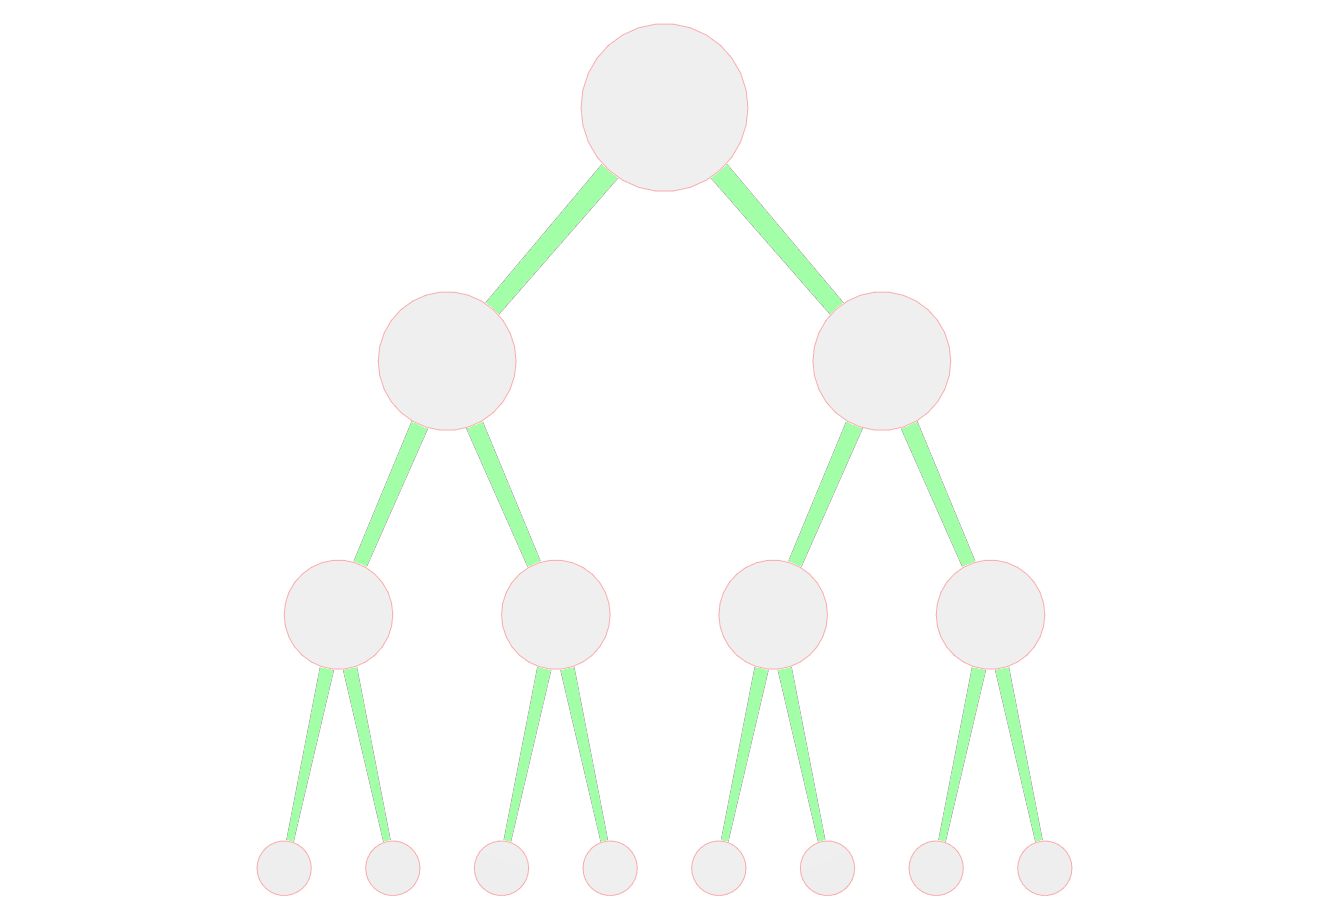
\includegraphics[width=11cm]{graphbintree3h.png}

\subsection{Non-Planar Graphs}

\subsubsection{Petersen Graph}

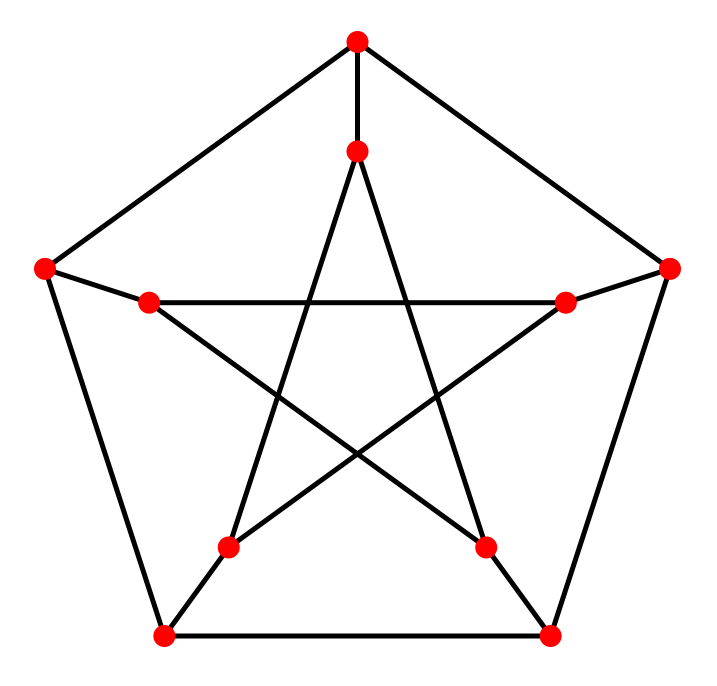
\includegraphics[width=11cm]{graphpetersen.png}

The Petersen graph is named for Julius Petersen, a famous Danish mathematician. The Petersen graph is a special case which is reputed to constitute a good counterexample to many theories that work on other graphs. 

\subsubsection{Icosahedron Graph}

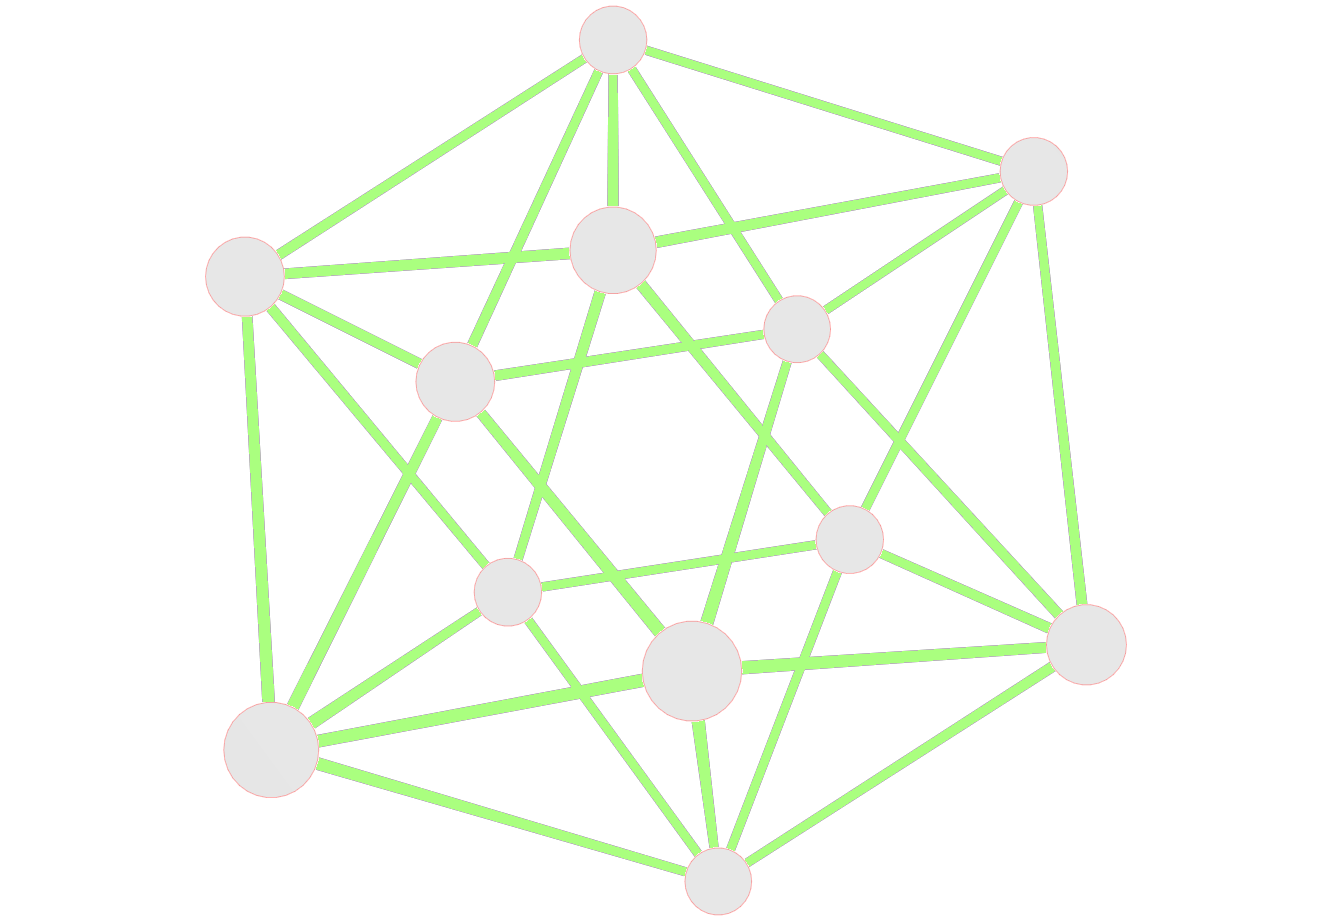
\includegraphics[width=11cm]{graphicosaedre.png}

The Icosahedron is often found in biology in viral structures. We are interested in the particular topology.